\documentclass[../notes.tex]{subfiles}

\pagestyle{main}
\renewcommand{\chaptermark}[1]{\markboth{\chaptername\ \thechapter\ (#1)}{}}
\setcounter{chapter}{8}

\begin{document}




\chapter{Rigid Body Motion}
\section{Introduction; Rotation About an Axis; Moments of Inertia}
\begin{itemize}
    \item \marginnote{11/3:}Announcements.
    \begin{itemize}
        \item We will now have \emph{seven} problem sets instead of \emph{eight}.
        \begin{itemize}
            \item Each problem set is now worth more (PSets still amount to 40\% of our grade).
            \item There will still be one makeup PSet at the end of the quarter.
        \end{itemize}
        \item PSet 5 is due next Friday.
    \end{itemize}
    \item Recap: Many-body motion.
    \begin{itemize}
        \item It's useful to introduce the center of mass coordinate, $\vec{R}=1/M\cdot\sum_\alpha m_\alpha\vec{r}_\alpha$, where $M=\sum_\alpha m_\alpha$.
        \item In the CM frame, $\vec{R}{\,}^*=0$ and $\vec{r}_\alpha=\vec{R}+\vec{r}_\alpha{}^*$.
        \begin{itemize}
            \item We also have $\vec{P}{\,}^*=0$, $T^*=\sum_\alpha m_\alpha(\dot{\vec{r}}_\alpha{}^*)^2/2$, and $\vec{J}{\,}^*=\sum_\alpha m_\alpha\vec{r}_\alpha{}^*\times\dot{\vec{r}}_\alpha{}^*$.
        \end{itemize}
        \item Then, going back into the lab frame, we have $\vec{P}=M\cdot\dot{\vec{R}}$, $T=M\dot{\vec{R}}^2/2+T^*$, and $\vec{J}=M\vec{R}\times\dot{\vec{R}}+\vec{J}{\,}^*$.
        \item One more note before we move onto rigid bodies: Suppose we're interested in the work, i.e., the rate of change of $T$ in the system.
        \begin{itemize}
            \item Recall that $m\ddot{\vec{r}}_\alpha=\sum_\beta\vec{F}_{\alpha\beta}+\vec{F}_\alpha$.
            \item Thus,
            \begin{equation*}
                \dot{T} = \sum_\alpha m_\alpha\dot{\vec{r}}_\alpha\cdot\ddot{\vec{r}}_\alpha
                = \sum_\alpha\sum_\beta\dot{\vec{r}}_\alpha\cdot\vec{F}_{\alpha\beta}+\sum_\alpha\dot{\vec{r}}_\alpha\cdot\vec{F}_\alpha
            \end{equation*}
            \item Note: Even letting $\vec{r}_{\alpha\beta}=\vec{r}_\alpha-\vec{r}_\beta$ and using $\vec{F}_{\alpha\beta}=-\vec{F}_{\beta\alpha}$, the left term above is often not equal to zero, i.e., there is no reason for it to vanish as in previous cases.
            \begin{itemize}
                \item This is not surprising, as it makes sense that the internal potential energy of the system would change in many cases.
            \end{itemize}
            \item However, if the $\vec{F}_{\alpha\beta}$ are conservative, then
            \begin{equation*}
                \dot{\vec{r}}_{\alpha\beta}\cdot\vec{F}_{\alpha\beta} = -\dv{t}V_{\text{int},\alpha\beta}
            \end{equation*}
            is the rate of internal forces doing work.
            \item Consequence: The rate of change of the kinetic plus internal potential energy is equal to the rate at which the external forces do work. That is,
            \begin{equation*}
                \dv{t}(T+V_\text{int}) = \sum_\alpha\dot{\vec{r}}_\alpha\cdot\vec{F}_\alpha
            \end{equation*}
            \item Additionally, we can find the rate of change of energy relative to the center of mass. In particular, in the CM frame, we have
            \begin{equation*}
                \dv{t}(\frac{1}{2}M\dot{\vec{R}}^2) = M\dot{\vec{R}}\cdot\ddot{\vec{R}}
                = \dot{\vec{R}}\cdot\sum_\alpha\vec{F}_\alpha
            \end{equation*}
            \item Subtracting the above equation from the one above it, we obtain
            \begin{align*}
                \dv{t}(T^*+V_\text{int}) &= \dv{t}(T-\frac{1}{2}M\dot{\vec{R}}^2+V_\text{int})\\
                &= \sum_\alpha\dot{\vec{r}}_\alpha\cdot\vec{F}_\alpha-\dot{\vec{R}}\cdot\sum_\alpha\vec{F}_\alpha\\
                &= \sum_\alpha\dot{\vec{r}}_\alpha{}^*\cdot\vec{F}_\alpha
            \end{align*}
            \item Note that in the leftmost term above, we are differentiating the total energy in the CM frame with respect to time. But since the time rate of change of energy is power, what we have expressed is the power.
        \end{itemize}
        \item Comparing this to $\dot{\vec{J}}{\,}^*=\sum_\alpha\vec{r}_\alpha{}^*\times\vec{F}_\alpha$, we see that we have a similar structure.
    \end{itemize}
    \item Today.
    \begin{itemize}
        \item Rigid bodies (a special case of many-body motion in which the particles are fixed relative to each other).
        \item Motion about an axis.
    \end{itemize}
    \item Today, we will primarily focus on rotation about an axis.
    \item The setup is as follows.
    \begin{itemize}
        \item We choose rotation to be in the $\hat{z}$ direction. We choose a shape (whatever we want), and it is rotating about this $\hat{z}$ axis.
        \item If is often useful to use cylindrical coordinates $(\rho,\phi,z)$ here because of the axial symmetry.
        \begin{itemize}
            \item Conversions: $x=\rho\cos\phi$, $y=\rho\sin\phi$, and $z=z$.
            \item Note that $\vec{r}=z\hat{z}+\rho\hat{\rho}$, much like in Figure \ref{fig:Vrotation}.
        \end{itemize}
        \item Recall that $\dv*{\vec{r}}{t}=\vec{\omega}\times\vec{r}=\dot{\vec{r}}$.
        \item We can now calculate our $\vec{J}$. It is equal to
        \begin{equation*}
            \vec{J} = \sum_\alpha m_\alpha\vec{r}_\alpha\times\dot{\vec{r}}_\alpha
            = \sum_\alpha m_\alpha\vec{r}_\alpha\times(\vec{\omega}\times\vec{r}_\alpha)
        \end{equation*}
        \item Expanding out the cross product, we obtain
        \begin{equation*}
            \begin{pmatrix}
                \hat{\rho} & \hat{\phi} & \hat{z}\\
                0 & 0 & \omega\\
                \rho & 0 & z\\
            \end{pmatrix}
            = \omega\rho\hat{\phi}
        \end{equation*}
        \item Expanding out our second cross product, we obtain
        \begin{equation*}
            \begin{pmatrix}
                \hat{\rho} & \hat{\phi} & \hat{z}\\
                \rho & 0 & z\\
                0 & \rho\omega & 0\\
            \end{pmatrix}
            = -z\rho\omega\hat{\rho}+\rho^2\omega\hat{z}
        \end{equation*}
    \end{itemize}
    \item Thus, we have that
    \begin{align*}
        \vec{J} &= \sum_\alpha m_\alpha(\rho_\alpha^2\omega\hat{z}-z_\alpha\omega\rho_\alpha\hat{\rho})\\
        &= \sum_\alpha m_\alpha[\rho_\alpha^2\omega\hat{z}-z_\alpha\omega(\rho_\alpha\cos\phi\hat{x}+\rho_\alpha\sin\phi\hat{y})]\\
        &= \omega\left( \sum_\alpha m_\alpha\rho_\alpha^2 \right)\hat{z}-\left( \omega\sum_\alpha m_\alpha z_\alpha x_\alpha \right)\hat{x}-\left( \omega\sum_\alpha m_\alpha z_\alpha y_\alpha \right)\hat{y}
    \end{align*}
    \begin{itemize}
        \item We can get this into a more familiar term via \textbf{moments of inertia}.
    \end{itemize}
    \item \textbf{Moment of inertia} (about the $z$-axis). \emph{Denoted by} $\bm{I_{zz}}$. \emph{Given by}
    \begin{equation*}
        I_{zz} = \sum_\alpha m_\alpha\rho_\alpha^2
        = \sum_\alpha m_\alpha(x_\alpha^2+y_\alpha^2)
    \end{equation*}
    \begin{itemize}
        \item In general, these are \textbf{second} moments about an axis. This just reflects the fact that the axial distance is \emph{squred}.
    \end{itemize}
    \item \textbf{Products of inertia}. Examples.
    \begin{itemize}
        \item $I_{xz}=-\sum_\alpha m_\alpha x_\alpha z_\alpha$.
        \item $I_{yz}=-\sum_\alpha m_\alpha y_\alpha z_\alpha$.
    \end{itemize}
    \item It follows from these definitions that, for $\vec{\omega}=\omega\hat{z}$, we have
    \begin{align*}
        J_z &= I_{zz}\omega&
        J_y &= I_{yz}\omega&
        J_x &= I_{xz}\omega
    \end{align*}
    \begin{itemize}
        \item Note that if $\vec{\omega}=\omega\hat{x}$, we have
    \end{itemize}
    \begin{align*}
        J_z &= I_{zx}\omega&
        J_y &= I_{yx}\omega&
        J_x &= I_{xx}\omega
    \end{align*}
    \item If we have $\vec{\omega}=\omega_x\hat{x}+\omega_y\hat{y}+\omega_z\hat{z}$, then the contributions to angular momentum add via
    \begin{equation*}
        \begin{bmatrix}
            J_x\\
            J_y\\
            J_z\\
        \end{bmatrix}
        = \underbrace{
            \begin{bmatrix}
                I_{xx} & I_{xy} & I_{xz}\\
                I_{yx} & I_{yy} & I_{yz}\\
                I_{zx} & I_{zy} & I_{zz}\\
            \end{bmatrix}
        }_I
        \begin{bmatrix}
            \omega_x\\
            \omega_y\\
            \omega_z\\
        \end{bmatrix}
    \end{equation*}
    \begin{itemize}
        \item $I$ is the \textbf{moment of inertia tensor}.
        \item It follows that, for example,
        \begin{equation*}
            J_x = I_{xx}\omega_x+I_{xy}\omega_y+I_{xz}\omega_z
        \end{equation*}
    \end{itemize}
    \item What's a tensor?
    \begin{itemize}
        \item It's like a matrix with a tiny bit more structure.
        \item For now, think of it as a $3\times 3$ matrix, and we'll talk more about it a little bit more next time.
    \end{itemize}
    \item Consider again $\vec{\omega}=\omega\hat{z}$.
    \begin{itemize}
        \item Then
        \begin{equation*}
            J_z = I_{zz}\omega
            = \sum_\alpha m_\alpha\rho_\alpha^2\omega
        \end{equation*}
        \item It follows that
        \begin{equation*}
            \dot{\vec{J}} = \sum_\alpha\vec{r}_\alpha\times\vec{F}_\alpha
        \end{equation*}
        \item Computing the cross product, we have
        \begin{equation*}
            \begin{pmatrix}
                \hat{\rho} & \hat{\phi} & \hat{z}\\
                \rho_\alpha & 0 & z_\alpha\\
                F_\rho & F_\phi & F_z\\
            \end{pmatrix}
            = -F_\phi z_\alpha\hat{\rho}+\rho_\alpha F_\phi\hat{z}
        \end{equation*}
        \item Then
        \begin{equation*}
            \dot{J}_z = I_{zz}\dot{\omega}
            = \sum_\alpha\rho_\alpha F_\phi
        \end{equation*}
        \begin{itemize}
            \item This is the equation of motion for rigid bodies.
            \item It gives $\omega(t)$ in terms of force $F_\phi$.
        \end{itemize}
    \end{itemize}
    \item Example: Equilibrium.
    \begin{figure}[h!]
        \centering
        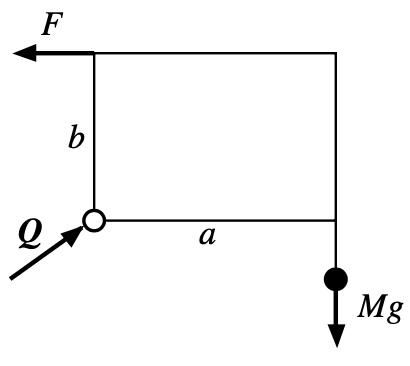
\includegraphics[width=0.22\linewidth]{../ExtFiles/rectangularLamina.png}
        \caption{The rectangular lamina.}
        \label{fig:rectangularLamina}
    \end{figure}
    \begin{itemize}
        \item The \textbf{rectangular lamina}.
        \item We're pulling on two corners, and if it's in equilibrium, the thing is not rotating. This means that
        \begin{align*}
            bF-aMg &= 0\\
            F &= \frac{a}{b}Mg
        \end{align*}
    \end{itemize}
    \item Kinetic energy.
    \begin{itemize}
        \item We have that
        \begin{equation*}
            T = \sum_\alpha\frac{1}{2}m_\alpha(\rho_\alpha\omega)^2
            = \frac{1}{2}I\omega^2
        \end{equation*}
        \item It follows that the time rate of change of the kinetic energy is
        \begin{equation*}
            \dot{T} = I\omega\dot{\omega}
            = \sum_\alpha\omega\rho_\alpha F_\phi
            = \sum_\alpha(\rho\dot{\phi})F_\phi
            = \sum_\alpha\dot{\vec{r}}_\alpha\cdot\vec{F}_\alpha
        \end{equation*}
        \item Thus, in this case, the internal forces do no work (which in some sense makes sense for a rigid body).
        \item Thus, the KE is just related to these external forces as shown above.
    \end{itemize}
    \item We'll talk about pivot points next time.
\end{itemize}



\section{Euler's Angles; Freely Rotating Symmetric Body}
\begin{itemize}
    \item \marginnote{11/6:}Announcements.
    \begin{itemize}
        \item Our exams are graded; we can pick them up after class.
        \begin{itemize}
            \item High: 96\%.
            \item Median: 71\%.
        \end{itemize}
        \item Our course grades will be curved.
        \begin{itemize}
            \item $\text{A}^-$/$\text{B}^+$ cutoff is likely 83\%.
            \item $\text{B}^-$/$\text{C}^+$ cutoff is likely 60\%.
        \end{itemize}
        \item Office hours are back in her office today.
        \item Where we're going.
        \begin{itemize}
            \item Next week: Hamiltonians and conservation laws.
            \item Then Thanksgiving.
            \item Then a bit of dynamical systems.
        \end{itemize}
    \end{itemize}
    \item Recap.
    \begin{itemize}
        \item Rigid bodies --- rotation about a fixed axis.
        \item Moments and products of inertia.
        \begin{itemize}
            \item What is a tensor?
        \end{itemize}
    \end{itemize}
    \item Addressing a question from last time: Why do we call $T^*+V_\text{int}$ the "total energy" in the CM frame?
    \begin{itemize}
        \item It's tautological: This is the only possible definition of "total energy" in the CM frame.
        \item More specifically, recall that $\dv*{t}(T+V_\text{int})=\sum_\alpha\dot{\vec{r}}_\alpha\cdot\vec{F}_\alpha$ and $\dv*{t}(T^*+V_\text{int})=\sum_\alpha\dot{\vec{r}}_\alpha{}^*\cdot\vec{F}_\alpha$.
        \begin{itemize}
            \item If the $\vec{F}_\alpha$ are \emph{conservative}, then we can define $V_\text{ext}$ via
            \begin{equation*}
                -\dv{t}(V_\text{ext}(\{\vec{r}_\alpha\})) = -\sum_{\alpha,i}\pdv{V_\text{ext}}{r_{\alpha i}}\dv{r_{\alpha i}}{t}
                = -\sum_\alpha\dot{\vec{r}}_\alpha\cdot\vec{F}_\alpha
            \end{equation*}
            \item Plugging the above into the expression for $\dv*{t}(T+V_\text{int})$ given above yields
            \begin{equation*}
                \dv{t}(T+V_\text{int}+V_\text{ext}) = 0
            \end{equation*}
            \item But this is exactly the condition we expect for \emph{conservative} external forces.
        \end{itemize}
        \item Visualizing the system also helps make this definition of total energy more clear.
        \begin{itemize}
            \item Recall that the system is like a bunch of particles connected by springs, all of which are connected to some external potential like gravity.
            \item When we talk about the "total energy" in the CM frame, we're essentially just "diagonalizing" the system between external and internal forces.
        \end{itemize}
    \end{itemize}
    \item Back to rigid bodies now.
    \item Rigid body motion is completely specified by the following two equations of motion.
    \begin{enumerate}
        \item $\dot{\vec{P}}=M\ddot{\vec{R}}=\sum_\alpha\vec{F}_\alpha$.
        \begin{itemize}
            \item Looks like a particle of mass $M$ at the CM.
        \end{itemize}
        \item $\dot{\vec{J}}=\sum_\alpha\vec{r}_\alpha\times\vec{F}_\alpha$.
    \end{enumerate}
    \item Recap.
    \begin{itemize}
        \item Last time, we found that there's a huge simplification we can make because all the particles in a rigid body are locked together.
        \begin{itemize}
            \item The simplification is that $\vec{J}=\overleftrightarrow{I}\vec{\omega}$, where $\overleftrightarrow{I}$ is the moment of inertia tensor from last time.
            \item Jerison writes out the matrix formula all over again.
            \item Point to emphasize: $\overleftrightarrow{I}$ is an intrinsic property of the rigid body, and it plays the role of mass.
            \item If we have a continuous object, the sums over indices $\alpha$ turn into an integral! Recall this from prior courses.
            \item Compare to $\vec{P}=M\dot{\vec{R}}$ to see that there is a similar structure in the above equation.
        \end{itemize}
        \item Special case: Rotation about a fixed axis.
        \begin{itemize}
            \item We're headed toward the \textbf{compound pendulum}.
            \item For such a problem, we use cylindrical coordinates.
            \begin{itemize}
                \item Jerison redefines the coordinate conversions.
            \end{itemize}
            \item We take $\vec{\omega}$ to lie in the $\khat$ direction via $\vec{\omega}=\omega\khat$.
            \item The moment we're most concerned with is $I_{zz}$, defined as previously. Differentiating gets us to $J_z=I_{zz}\omega_z$ and $\dot{J}_z=I_{zz}\dot{\omega}$.
            \item From here, we can define the kinetic energy
            \begin{equation*}
                T = \sum_\alpha\frac{1}{2}m_\alpha\dot{\vec{r}}_\alpha{}^2
                = \sum_\alpha\frac{1}{2}m_\alpha(\rho_\alpha\omega)^2
                = \frac{1}{2}I_{zz}\omega^2
            \end{equation*}
            where we recall that $\dot{\vec{r}}_\alpha=\vec{\omega}\times\vec{r}_\alpha=\rho_\alpha\omega\,\hat{\phi}$.
        \end{itemize}
    \end{itemize}
    \item The EOMs for this system are given by $\dot{\vec{J}}=\sum_\alpha\vec{r}_\alpha\times\vec{F}_\alpha$.
    \begin{itemize}
        \item We're mostly interested in the $z$ component, i.e., $\dot{J}_z=\sum_\alpha\rho_\alpha F_\phi$.
        \item Sometimes, it can be useful to separate out the forces into axial forces and other forces via
        \begin{equation*}
            \dot{\vec{P}} = M\ddot{\vec{R}}
            = \vec{Q}+\sum_\alpha\vec{F}_\alpha
        \end{equation*}
        \item To make calculations, it will additionally be useful to have the following expression. For a rotating body, $\dot{\vec{R}}$ is given via $\dot{\vec{R}}=\vec{\omega}\times\vec{R}$ and $\ddot{\vec{R}}=\dot{\vec{\omega}}\times\vec{R}+\vec{\omega}\times\dot{\vec{R}}=\dot{\vec{\omega}}\times\vec{R}+\vec{\omega}\times(\vec{\omega}\times\vec{R})$.
    \end{itemize}
    \item This is true in general; if we specialize to our case of rotation about an axis\dots
    \begin{itemize}
        \item We first choose coordinates such that $z_\text{cm}=0$.
        \item Since this is rotation about an axis, the above equation simplifies to
        \begin{equation*}
            \ddot{\vec{R}} = R\dot{\omega}\,\hat{\phi}-\omega^2R\,\hat{\phi}
            = R\ddot{\phi}\,\hat{\phi}-\dot{\phi}^2R\,\hat{\rho}
        \end{equation*}
        \item In the right term above, the left term is tangential acceleration and the right term is centripetal acceleration.
    \end{itemize}
    \item Example: Compound pendulum.
    \begin{figure}[h!]
        \centering
        \begin{tikzpicture}
            \small
            \draw [stealth-stealth] (2,0) node[right]{$y$} -- (0,0) coordinate (o) -- (0,-2) coordinate (x) node[below]{$x$};
            \fill circle (1.5pt);
    
            \footnotesize
            \coordinate (c) at (-50:0.8);
            \draw [pux,thick,rotate around={-50:(c)}] (c) ellipse (1.5cm and 1cm);
            \draw [->] (0,0) -- node[right,yshift=1mm]{$\vec{R}$} (c);
            \draw [->] (c) -- node[right]{$\vec{F}$} ++(0,-1);
            \pic [draw,angle radius=4mm,angle eccentricity=1.4,pic text={$\phi$}] {angle=x--o--c};
        \end{tikzpicture}
        \caption{Compound pendulum.}
        \label{fig:compoundPendulum}
    \end{figure}
    \begin{itemize}
        \item We want to look at the force on the pivot.
        \item We define a new coordinate system as in Figure \ref{fig:compoundPendulum}. Explicitly, $\hat{x}$ points straight downwards and $\hat{y}$ points straight rightwards.
        \item We put our pendulum's center of mass such that it rotates through angle $\phi$.
        \item At this point, we have
        \begin{align*}
            T &= \frac{1}{2}I_{zz}\dot{\phi}^2&
            V &= M\vec{g}\cdot\vec{R} = -MgR\cos\phi
        \end{align*}
        \item Thus, our Lagrangian is
        \begin{equation*}
            L = T-V = \frac{1}{2}I_{zz}\dot{\phi}^2+MgR\cos\phi
        \end{equation*}
        \item It follows that our EOM is
        \begin{align*}
            I\ddot{\phi} &= -MgR\sin\phi\\
            \ddot{\phi} &= -\frac{MgR}{I}\sin\phi\\
            &= -\frac{g}{\ell}\sin\phi
        \end{align*}
        where $\ell=I/MR$.
        \begin{itemize}
            \item $\ell$ defines the \textbf{equivalent simple pendulum}.
        \end{itemize}
        \item From here, we can solve for the force on the pivot as a function of $\phi$ (we could also go through $\phi(t)$, and solve for $F(t)$ if we desired).
        \begin{itemize}
            \item We start with the conservation of energy
            \begin{equation*}
                \frac{1}{2}I\dot{\phi}^2-MgR\cos\phi = E
            \end{equation*}
            \item It follows that
            \begin{equation*}
                \dot{\phi}^2 = \frac{E+MgR\cos\phi}{I/2}
                = \frac{2E}{Mr\ell}+\frac{2g}{\ell}\cos\phi
            \end{equation*}
            \item We want to solve for $\vec{Q}$ from $M\ddot{\vec{R}}=\vec{Q}+\sum_\alpha\vec{F}_\alpha$.
            \item Here, the only relevant external force is our gravitational force $Mg\cos\phi\,\hat{\rho}-Mg\sin\phi\,\hat{\phi}$.
            \item We also found previously that $\ddot{\vec{R}}=R\ddot{\phi}\,\hat{\phi}-\dot{\phi}^2R\,\hat{\rho}$. Thus,
            \begin{equation*}
                MR\ddot{\phi}\,\hat{\phi}-MR\dot{\phi}^2\,\hat{\rho} = \vec{Q}+Mg\cos\phi\,\hat{\rho}-Mg\sin\phi\,\hat{\phi}
            \end{equation*}
            \item Splitting this vector equation into scalar equations, we obtain
            \begin{align*}
                Q_\rho &= -MR\dot{\phi}^2-Mg\cos\phi&
                Q_z &= 0&
                Q_\phi &= MR\ddot{\phi}+Mg\sin\phi
            \end{align*}
            \item Substituting from the conservation of energy, we obtain
            \begin{align*}
                Q_\rho &= -\frac{2E}{\ell}-Mg\left( 1+\frac{2R}{\ell} \right)\cos\phi&
                Q_z &= 0&
                Q_\phi &= Mg\left( 1-\frac{R}{\ell} \right)\sin\phi
            \end{align*}
            \item These are the final formulae for the forces on pivot as a function of $\phi$.
        \end{itemize}
    \end{itemize}
    \item \textbf{Equivalent simple pendulum}: The simple pendulum having the same equation of motion as our extended body.
    \item What happens in a similar system when we have a "sudden blow" or impulse?
    \begin{figure}[h!]
        \centering
        \begin{tikzpicture}
            \small
            \draw [stealth-stealth] (2,0) node[right]{$y$} -- (1.5,0) -- (1.5,-0.5) node[below]{$x$};
            \node at (1.7,-0.2) {$+$};
    
            \footnotesize
            \fill
                (0,0) circle (1.5pt)
                (0,-1.6) circle (1.5pt)
            ;
            \coordinate (c) at (0,-0.8);
            \draw [pux,thick,rotate around={-90:(c)}] (c) ellipse (1.5cm and 1cm);
            \draw [dashed] (0,0) -- node[right]{$d$} ($(0,0)!2!(c)$);
    
            \draw [->] (-2.3,-1.6) -- node[above]{$\vec{K}$} ++(0.9,0);
            \draw [->,shorten >=2pt] (0.7,0) -- node[above]{$\vec{S}$} (0,0);
        \end{tikzpicture}
        \caption{The "sweet spot" of a compound pendulum.}
        \label{fig:compoundPendulum2}
    \end{figure}
    \begin{itemize}
        \item Such pendulums have a sweet spot or equilibrium where the CM is just hanging down.
        \item We imagine that we kick the pendulum with impulse $\vec{K}$ in the $\hat{y}$ direction (using our modified coordinate system), as shown above.
        \item We have that $K\hat{y}=\vec{K}=\vec{F}\Delta t$.
        \item Let $\vec{S}=\vec{Q}\Delta t$.
        \item What we'll see is that there is a special value of $d$ (between the pivot and CM) for which $\vec{\rho}$ vanishes!
        \item During the short interval,
        \begin{equation*}
            I\ddot{\phi} = -MgR\sin\phi+Fd
        \end{equation*}
        \item We make the approximation that $\ddot{\phi}$ is constant during $\Delta t$ and that $\sin\phi=0$.
        \item It follows that
        \begin{equation*}
            \omega_\text{final} = \ddot{\phi}\Delta t
            = F\Delta t\frac{d}{I}
            = \frac{Kd}{I}
        \end{equation*}
        \item Additionally, we have that $\dot{\vec{P}}=\vec{Q}+\vec{F}$ so that
        \begin{equation*}
            P_\text{final} = \dot{P}\Delta t
            = -Q\Delta t+F\Delta t
            = -S+K
        \end{equation*}
        \item But we also know that
        \begin{equation*}
            P_\text{final} = M\dot{R}_\text{final}
            = M\omega_\text{final}R
            = \frac{MKdR}{I}
        \end{equation*}
        \item Thus, putting everything together, we obtain
        \begin{align*}
            \frac{MKdR}{I} &= -S+K\\
            S &= K\left( 1-\frac{MdR}{I} \right)
        \end{align*}
        \item Thus, $S$ vanishes if we choose $d=\ell=I/MR$.
        \item Takeaway: Regardless of the shape of our pendulum, if we hit it at the distance of the equivalent simple pendulum, we'll have no impulse on the pivot.
        \item This is the "sweet spot" of our baseball bat or whatever.
    \end{itemize}
\end{itemize}



\section{Office Hours (Jerison)}
\begin{itemize}
    \item \marginnote{11/6:}The final will slant toward the second half of the course, but everything is fair game.
    \item Is there an abstract environment in which we can view mass vs. angular mass and momentum vs. angular momentum, etc. as special cases of the same generalized construct?
    \begin{itemize}
        \item Yes.
        \item One answer.
        \begin{itemize}
            \item We can get this mapping from a speed-type thing to a momentum-type thing with linear operators.
            \item A tensor is a mathematical object with some kind of geometrical meaning independent of the coordinate basis.
        \end{itemize}
        \item Another answer.
        \begin{itemize}
            \item These are both examples of equations of motion that come from the Lagrangian (think \emph{generalized} mass, \emph{generalized} momentum, \emph{generalized} force, etc.).
        \end{itemize}
    \end{itemize}
    \item Could you post the KE of a free particle derivation?
    \item There will not be another \emph{in-class} review session, but she will hold one outside of class.
    \item We will get to Euler angles on Friday.
\end{itemize}



\section{Moment of Inertia Tensor; Principal Axis Rotation}
\begin{itemize}
    \item \marginnote{11/8:}Outline.
    \begin{itemize}
        \item Moment of inertia tensor.
        \begin{itemize}
            \item What is a tensor?
            \item Principal axes.
            \item Calculating moments of inertia.
        \end{itemize}
        \item Rotation about a principal axis.
        \begin{itemize}
            \item Precession.
        \end{itemize}
    \end{itemize}
    \item Next time.
    \begin{itemize}
        \item Stability of rotation about a principal axis.
        \item Euler angles.
        \item Lagrangian for rigid bodies.
    \end{itemize}
    \item Recall.
    \begin{itemize}
        \item Our EOMs are
        \begin{align*}
            \dot{\vec{P}} &= M\ddot{\vec{R}} = \sum_\alpha\vec{F}_\alpha&
            \dot{\vec{J}} &= \sum_\alpha\vec{r}_\alpha\times\vec{F}_\alpha
        \end{align*}
        \item Last time, we talked about rotation about a fixed axis.
        \item We've also seen that more generally, if $\vec{\omega}=\omega_x\ihat+\omega_y\jhat+\omega_z\khat$, then the angular momentum is given by
        \begin{equation*}
            \vec{J} = \overleftrightarrow{I}\vec{\omega}
        \end{equation*}
    \end{itemize}
    \item \textbf{Tensor}: A mathematical object that has geometric meaning independent of the coordinate basis.
    \item What is a tensor?
    \begin{itemize}
        \item She won't belabor the point because most of this machinery is orthogonal to our present aims.
        \item The "geometric meaning" alluded to in the definition has to be some kind of multilinear relationship, usually between vectors.
        \item In particular, $\overleftrightarrow{I}$ is an intrinsic property of the rigid body and its geometry.
        \begin{itemize}
            \item Its \emph{numerical} representation will change with the basis, though.
        \end{itemize}
        \item To calculate it, we need to be able to define it in a particular basis.
        \begin{itemize}
            \item The tensor comes prepackaged with (1) a definition in one basis and (2) a rule about how to change bases.
        \end{itemize}
        \item So, in our specific example, $\overleftrightarrow{I}$ is the linear operator that takes $\vec{\omega}$ and returns to you $\vec{J}$ for your rigid body.
        \item The rule to calculate entries of $\overleftrightarrow{I}$ is: Start with the $3\times 3$ matrix and then employ
        \begin{align*}
            I_{xx} &= \iiint\rho_m(\vec{r})(z^2+y^2)&
            I_{xy} &= -\iiint\rho_m(\vec{r})xy&
        \end{align*}
        and the like where herein, $\rho_m$ is the density mass/volume, not the radial coordinate.
        \item Change of basis rule: If you have a change of basis matrix $R$, then $\overleftrightarrow{I}$ in your new basis looks like $R^{-1}IR$.
        \item Note that $\overleftrightarrow{I}$ is called a $\binom{1}{1}$ tensor since it has 1 \textbf{contravariant} and 1 \textbf{covariant} dimension, meaning that it is like a regular matrix with 1 dimension that transforms as row vectors and 1 dimension that transforms as column vectors.
        \item Other examples of tensors.
        \begin{itemize}
            \item Scalars: Rank 0 tensors (same in any dimension).
            \item Vectors: Rank 1 tensors (can be row or column vectors).
            \item Metrics: There are $\binom{0}{2}$ tensors which do \emph{not} transform as matrices, even though they are arrays of numbers.
        \end{itemize}
        \item Note that since $I_{xy}=I_{yx}$, etc., $\overleftrightarrow{I}$ is \textbf{symmetric}.
        \begin{itemize}
            \item This implies that $\overleftrightarrow{I}$ has three real eigenvalues.
            \item Moreover, the eigenvectors of $\overleftrightarrow{I}$ are orthogonal.
            \item Thus, the eigenvectors of $\overleftrightarrow{I}$ are called the \textbf{principal axes} $\vec{e}_1,\vec{e}_2,\vec{e}_3$. Thus, in principle, we can find these for any object we choose, even though in any object we study, it will be obvious which axes are which.
            \item In the special basis of the principal axes, $\overleftrightarrow{I}$ is diagonal, i.e., $\overleftrightarrow{I}=\diag(I_{xx},I_{yy},I_{zz})$. It follows that
            \begin{equation*}
                \vec{J} = I_1\omega_1\vec{e}_1+I_2\omega_2\vec{e}_2+I_3\omega_3\vec{e}_3
            \end{equation*}
        \end{itemize}
        \item We don't need to worry about any of this stuff if we don't want to.
    \end{itemize}
    \item All these tensor machinations help with defining\dots
    \begin{itemize}
        \item The kinetic energy as:
        \begin{equation*}
            T = \sum_\alpha\frac{1}{2}m_\alpha\dot{\vec{r}}_\alpha{}^2
            = \sum_\alpha\frac{1}{2}m_\alpha(\vec{\omega}\times\vec{r}_\alpha)^2
            = \sum_\alpha\frac{1}{2}m_\alpha[\omega^2r_\alpha^2-(\vec{\omega}\cdot\vec{r}_\alpha)^2]
        \end{equation*}
        \item The angular momentum as:
        \begin{equation*}
            \vec{J} = \sum_\alpha m_\alpha\vec{r}_\alpha\times\dot{\vec{r}}_\alpha
            = \sum_\alpha m_\alpha\vec{r}_\alpha\times(\vec{\omega}\times\vec{r}_\alpha)
            = \sum_\alpha m_\alpha[r_\alpha^2\vec{\omega}-(\vec{r}_\alpha\cdot\vec{\omega})\vec{r}_\alpha]
        \end{equation*}
        \item Comparing the above two results, we obtain
        \begin{equation*}
            T = \frac{1}{2}\vec{\omega}\cdot\vec{J}
        \end{equation*}
        \item In particular, in the basis of principal axes,
        \begin{equation*}
            T = \frac{1}{2}I_1\omega_1^2+\frac{1}{2}I_2\omega_2^2+\frac{1}{2}I_3\omega_3^2
        \end{equation*}
        \item We can use the above to get the Lagrangian for general rigid body motion.
        \item A few notes on this.
        \begin{itemize}
            \item $\vec{e}_1,\vec{e}_2,\vec{e}_3$ rotate with the body.
            \item $\vec{J}=\overleftrightarrow{I}\vec{\omega}$ implies that in general, $\vec{J}$ is not parallel to $\vec{\omega}$. However, if $\vec{\omega}$ is along $\vec{e}_1,\vec{e}_2,\vec{e}_3$, then $\vec{J}$ is parallel to $\vec{\omega}$.
        \end{itemize}
    \end{itemize}
    \item \textbf{Symmetric body}: A rigid body for which two of the moments of inertia (usually taken to be $I_1,I_2$) are equal.
    \item \textbf{Totally symmetric body}: A rigid body for which all three of the moments of inertia are equal.
    \item Examples of (totally) symmetric bodies.
    \begin{itemize}
        \item A cylinder and square pyramid are both symmetric.
        \item A sphere and cube are both totally symmetric.
    \end{itemize}
    \item We'll mostly be dealing with \emph{symmetric} bodies.
    \item In this case:
    \begin{itemize}
        \item We have that
        \begin{equation*}
            \vec{J} = I_1(\omega_1\vec{e}_1+\omega_2\vec{e}_2)+I_3\omega_3\vec{e}_3
        \end{equation*}
        \item Thus, any axis in place of $\vec{e}_1,\vec{e}_2$ is a principal axis; we can choose any pair of orthogonal vectors herein.
    \end{itemize}
    \item In the case of a totally symmetric object, any axis ais a principal axis and $\vec{J}$ is always parallel to $\vec{\omega}$.
    \item Calculating $\overleftrightarrow{I}$.
    \begin{enumerate}
        \item If we take $\vec{r}=\vec{R}+\vec{r}{\,}^*$, then
        \begin{equation*}
            \sum_\alpha m_\alpha x^* = \sum_\alpha m_\alpha y^* = \sum_\alpha m_\alpha z^* = 0
        \end{equation*}
        \begin{itemize}
            \item Let $\vec{R}=(X,Y,Z)$.
            \item The above identities imply that the cross terms work out as follows.
            \begin{equation*}
                I_{xy} = \sum_\alpha m_\alpha(X+x^*)(Y+y^*)
                = -MXY-\sum_\alpha m_\alpha x_\alpha^*y_\alpha^*
            \end{equation*}
            \item Similarly, for the moments of inertia,
            \begin{equation*}
                I_{xx} = M(Y^2+Z^2)+I_{xx}^*
            \end{equation*}
            \begin{itemize}
                \item This decomposes the moment of inertia into the sum of the moment of the CM about your origin and the moment of inertia relative to $\vec{R}$.
                \item This is the \textbf{parallel axis theorem}.
            \end{itemize}
        \end{itemize}
        \item Objects with 3 perpendicular symmetry planes.
        \begin{itemize}
            \item Picture a cylinder or an ellipsoid with uniform density and three axes $a,b,c$.
            \item Then
            \begin{align*}
                I_1^* &= M(\lambda_yb^2+\lambda_zc^2)&
                I_2^* &= M(\lambda_xa^2+\lambda_zc^2)&
                I_3^* &= M(\lambda_xa^2+\lambda_yb^2)
            \end{align*}
            where\dots
            \begin{itemize}
                \item $\lambda_x=\lambda_y=\lambda_z=1/5$ for an ellipsoid;
                \item $\lambda_x=\lambda_y=\lambda_z=1/3$ for a parallelipiped;
                \item $\lambda_x=\lambda_y=1/4$ and $\lambda_z=1/3$ for a cylinder.
            \end{itemize}
            \item The derivation of the above results is on \textcite[209-11]{bib:KibbleBerkshire}.
            \begin{itemize}
                \item We should look through this as we may be expected to do the integrals!
            \end{itemize}
            \item What are the $\lambda$'s?
            \begin{itemize}
                \item It's just a number that has to do with the geometry of the subscripted axis.
            \end{itemize}
        \end{itemize}
    \end{enumerate}
    \item An interesting case: The effect of a small force on an axis; \textbf{precession}.
    \begin{itemize}
        \item Imagine an object that is spinning fairly rapidly about one of its axes.
        \item Assume that we have a symmetric body and that initially, $\vec{\omega}=\omega\vec{e}_3$.
        \item It follows that initially, $\vec{J}=I_3\omega_3\vec{e}_3$.
        \item In the case of no external forces, we have
        \begin{equation*}
            \dot{\vec{J}} = I_3\dot{\vec{\omega}}_3
            = \sum\vec{r}_\alpha\times\vec{F}_\alpha
            = 0
        \end{equation*}
        \item Now imagine we exert a small force $\vec{F}$ at a distance $\vec{r}$ up the axis from the CM/origin.
        \item It follows that $\dot{\vec{J}}=I_3\dot{\vec{\omega}}=\vec{r}\times\vec{F}$.
        \item Thus, $\dot{\vec{J}}$ is perpendicular to $\vec{\omega}$ and $\vec{\omega}$ changes direction, so the system turns.
        \item Under gravity, the wheel turns right.
        \item \emph{Mysterious picture}
    \end{itemize}
    \item At this point, we can analyze the motion of a top/gyroscope!
    \begin{figure}[h!]
        \centering
        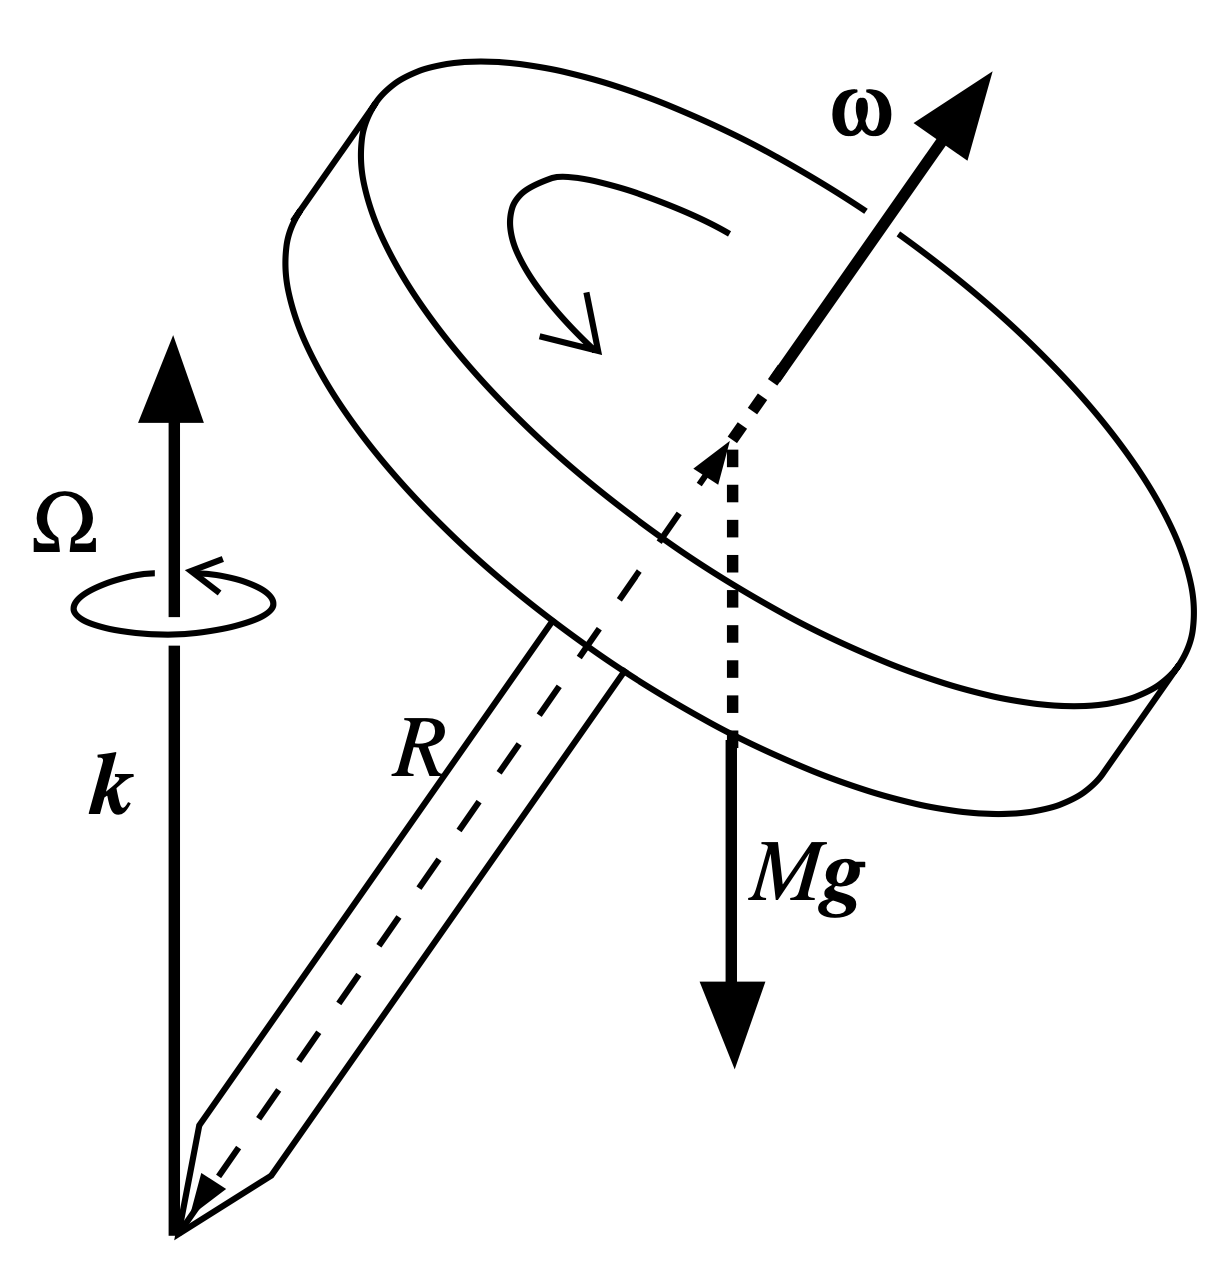
\includegraphics[width=0.2\linewidth]{../ExtFiles/topGyroscope.png}
        \caption{A spinning top/gyroscope.}
        \label{fig:topGyroscope}
    \end{figure}
    \begin{itemize}
        \item We have that
        \begin{align*}
            I_3\dot{\vec{\omega}} &= R\vec{e}_3\times(-Mg\khat)\\
            I_3\omega\dot{\vec{e}}_3 &= MgR\khat\times\vec{e}_3\\
            \dot{\vec{e}}_3 &= \frac{MgR}{I_3\omega}\khat\times\vec{e}_3
        \end{align*}
        \item Defining $\vec{\Omega}=\frac{MgR}{I_3\omega}\khat$, we have that
        \begin{equation*}
            \dot{\vec{e}}_3 = \vec{\Omega}\times\vec{e}_3
        \end{equation*}
        \item Thus, $\vec{e}_3$ rotates about the $\khat$ axis (direction of $\vec{\Omega}$) at rate $\Omega$. This is precession!
        \item We make the approximation that the value for $\Omega\ll\omega$, or $I_3\omega^2/2\gg MgR$.
        \item We are making the approximation that $\vec{J}$ points in the $\vec{\omega}$ direction ($\vec{e}_3$ direction), which is not quite true due to the $\Omega$ contribution.
    \end{itemize}
\end{itemize}



\section{Chapter 8: Many-Body Systems}
\emph{From \textcite{bib:KibbleBerkshire}.}
\begin{itemize}
    \item \marginnote{11/3:}Wrapping up Section 8.4.
\end{itemize}



\section{Chapter 9: Rigid Bodies}
\emph{From \textcite{bib:KibbleBerkshire}.}
\begin{itemize}
    \item Covered a smattering of results from various sections.
\end{itemize}




\end{document}